% -*- root: ../thesis.tex -*-

\chapter[The Future of a Missed Deadline]{The Future of a Missed Deadline}
% 
\label{ch:p01:ch02}
% 
\chapterauthor{Behrooz Nobakht, Frank S. de Boer, Mohammad Mahdi Jaghoori}

\section*{Abstract}
In this paper, we introduce a real-time actor-based programming language
and provide a formal but intuitive  operational semantics for it. 
The language supports a general mechanism for handling exceptions raised by missed deadlines
and the specification of application-level scheduling policies.
We discuss  the implementation of the language and 
illustrate the use of its constructs with an industrial case study from distributed e-commerce and marketing domain. 

\subparagraph*{Conference Publication}
\emph{Lecture Notes in Computer Science, Volume 7890, Coordination Models and Languages in 15th conference on Distributed Computing Techniques -- COORD 2013, Pages 181--195, DOI \smalltt{10.1007/978-3-642-38493-6\_13}}

% \keywords{actors, application-level scheduling, real-time, deadlines, futures, Java.}

\section{Introduction} \label{sec:introduction}

In real-time applications, rigid deadlines necessitate stringent scheduling strategies.
Therefore, the developer must ideally be able to program the scheduling of different tasks inside the application.
Real-Time Specification for Java (RTSJ) \cite{jsr1,jsr282} is a major extension of Java, as a mainstream programming language, aiming at enabling real-time application development. 
Although RTSJ extensively enriches Java with a framework for 
the  specification of real-time applications, 
it yet remains at the level of conventional \textit{multithreading}.
The drawback of multithreading is that it involves the programmer with OS-related concepts like threads, whereas a real-time Java developer should only be concerned about high-level entities, i.e., objects and method invocations, also with respect to 
real-time requirements.

The actor model \cite{fnd:actor:cmpt:agha} and actor-based programming languages, which
have re-emerged in the past few years \cite{kilim:Srinivasan:Mycroft,erlang:armstrong,scala:actors:ordersky,creol:broch:owe,salsa:agha}, 
provide a different and promising paradigm for concurrency and distributed computing, in which threads are transparently encapsulated inside actors.
As we will argue in this paper, this paradigm is much more suitable for real-time programming because it enables the programmer to 
obtain the appropriate   high-level view which allows the management of   complex
real-time requirements.

In this paper, we introduce an actor-based programming language Crisp for real-time applications. 
Basic real-time requirements include deadlines and timeouts.
In Crisp, deadlines are associated with asynchronous messages and timeouts  with futures \cite{BoerCJ07}.
Crisp further supports a general actor-based mechanism for handling exceptions raised by  missed deadlines.
By the  integration  of these basic real-time control mechanisms with the application-level policies supported by Crisp for scheduling of the messages inside an actor,
more complex real-time requirements of the application can be met with more flexibility and finer granularity.

We formalize the design of Crisp by means of structural  operational semantics \cite{plotkin:sos} and 
describe its implementation as a full-fledged programming language.
This implementation uses both the Java and Scala language with extensions of Akka library.
We illustrate the use of the programming language with an industrial case study from SDL Fredhopper that provides enterprise-scale distributed e-commerce solutions on the cloud.

% In previous work \cite{crisp-sac}, we presented a general framework, called Crisp, 
% to port the notion of {\em concurrent objects} from Creol \cite{creol:broch:owe,mpd:andrews} to Java. 
% A concurrent object encapsulates one processor, i.e., it has a
% single thread of execution. % that is controlled by the object itself.
% In other words, existing objects execute concurrently.
% In this setting, the thread of execution never leaves the enclosing object; instead, method invocations
% result in a new process inside the target object, i.e., they are asynchronous.  
% % Thus, a concurrent
% % object provides a natural basis for a deployment scheme where each
% % object virtually possesses one processor.
% Such a context brings the scheduling problem to the level of each active object in order to resolve the basic issue
% of which method in the object to select for execution.
% The Crisp framework introduces a scheduler for each object as a mathematical function on the values of different priority levels associated to each method definition, the current invocation or the caller.
% We concretize this idea in Crisp by allowing the developer to program a scheduler function inside each concurrent object definition.
% % This function can take as input the invocation deadline as well as other static and dynamic priorities associated to the method. 
% Additionally, active objects are able to use their own internal state to determine how the scheduling of 
% messages are done; this brings the problem of scheduling for real-time from low-level threads to the 
% level of objects and methods.
% 
% When message scheduling is elevated to the level of application inside the active object using the
% scheduler function, real-time requirements of the application can be met with more flexibility and finer granularity.
% Such real-time requirements include deadlines and timeouts. Using Crisp, each active object is able to
% take control of the different ways it behaves and reacts to deadlines and timeouts. Crisp allows the
% active object to define local timeouts in case the response is not received in due time. Additionally, 
% an active object may impose a deadline on the callee active object when sending a message to expect a response
% in a due time. Thus, Crisp provides seamless and direct mechanisms to meet real-time requirements
% at application level which relieves the programmer from many lower-level concerns.
% 
% 
% We extend our previous work \cite{crisp-sac} for Crisp. 
% Originally, Scala \cite{scala:actors:ordersky,coord:ordersky}, that runs on JVM, introduced a package
% for actor model programming. As an extension, Akka \cite{akka:homepage} extends Scala's actor library 
% with more facilities. We develop Crisp using both Java and Scala language with extensions of Akka library.
% In Crisp, actor features from Akka are extended and developed further to provide high- and application-level
% capabilities at the level of active objects to allow them take control of scheduling of the messages. 
% In Crisp, each active object may define a scheduler function while it may also use the notions of timeouts
% and deadlines when sending messages to other active objects. It is also possible to mix different scheduling
% mechanisms in Crisp which makes it more flexible for the active object in order to schedule message
% executions. The source code of Crisp along with previous work can be found at 
% \ftt{\url{http://github.com/nobeh/crisp}}.

The paper continues as follows: Section \ref{sec:deadlines} introduces the language constructs
and provides informal semantics of the language with a case study in Section \ref{sec:frh}. 
Section \ref{sec:sos} presents the operational semantics of Crisp.
Section \ref{sec:impl} follows to provide a detailed discussion on the implementation.
The case study continues in this section with further details and code examples.
Section \ref{sec:relwork} discusses related work of research and 
finally Section \ref{sec:conclusion} concludes the paper and proposes future line of research.

\section{Programming with deadlines} \label{sec:deadlines}
In this section, we introduce the basic concepts underlying  the notion of ``deadlines'' for asynchronous messages between actors. 
The main new constructs specify how a message can be sent with a deadline, how the message response can be processed, and what happens when a deadline is missed.
We discuss the informal semantics of these concepts  and illustrate them using a case study in Section \ref{sec:frh}.

Listing \ref{fig:grammar} introduces a minimal version of the  real-time
actor-based language Crisp.
Below we discuss the two main new language constructs presented at lines (7) and (8).
% In Line (6), we introduce an extension on how each concurrent object can send a message to another concurrent object annotated with an extra
% property that represents a deadline ($d$). 

\begin{figure}[t]
\begin{align}
C &::= \textbf{\jtt{class}} \; \mathsf{N} \; \textbf{\jtt{begin}} \; V^? \; \{M\}^* \; \textbf{\jtt{end}} \\
M_{sig} &::=
%\textbf{\jtt{op}} \; 
\mathsf{N}(\overline{T \: x}) \\ 
M &::= \{ M_{sig} == \{V \; ;\}^? S \} \\
V &::= \textbf{\jtt{var}} \; \{\{x\},^+ \; : \; \mathsf{T} \; \{ = e\}^? \},^+ \\
S &::=  x := e\; | \\
 &::= x := \textbf{\jtt{new}} \; \mathsf{T}(e^?) \; |\\
&:= f = e \; ! \; m(\overline{e}) \; \textbf{\jtt{deadline}}(e) \: | \\
 &::= x := f.\gett(e^?) \; | \\
  &::= \textbf{\jtt{return}} \; e  \; | \\
  &::= S \; ; \; S \; | \\
  &::= \textbf{\jtt{if}} \; (b) \; \textbf{\jtt{then}} \; S \; \textbf{\jtt{else}} \; S \; \textbf{\jtt{end}}  \; | \\
  &::= \textbf{\jtt{while}} \; (b) \; \{ \; S \; \} \; | \\
  &::= \textbf{\jtt{try}} \: \{ S \} \: \jtt{\textbf{catch}}(\mathsf{T}_{\jtt{Exception}} \; x) \: \{ \: S \: \}  
%E &::= B \; | \; V \\
%B &::= \textbf{\jtt{true}} \; | \; \textbf{\jtt{false}} \; | \; B \wedge B \; | \; B \vee B \; | \; %\textbf{\jtt{not}} \; B
\end{align}
\caption{
A kernel version of the real-time programming language.
The bold scripted \textbf{\jtt{keywords}} denote the reserved words in the language.
The over-lined $\overline{v}$ denotes a sequence  of syntactic entities $v$.
Both local and instance variables are denoted by $x$.
We assume distinguished local variables  $\jtt{this}$, $\jtt{myfuture}$, and  $\jtt{deadline}$ which
denote the actor itself, the  unique future corresponding to the process, and  its deadline,  respectively.
A distinguished instance variable $\jtt{time}$  denotes  the current time.
Any subscripted type $\mathsf{T}_{specialized}$ denotes a \textit{specialized} type of general type $\mathsf{T}$; 
e.g. $\mathsf{T}_{\jtt{Exception}}$ denotes all ``exception'' types.
A variable $f$ is in $\mathsf{T}_{future}$. 
\textsf{N} is a name (identifier) used for classes and method names.
%$e$ is in \textsf{Expression} ($E$);
$C$ denotes a class definition which consists of  a definition of its instance variables
and its methods;
$M_{sig}$ is a method signature; $M$ is a method definition; $S$ denotes a statement.
We abstract from the syntax the side-effect free expressions $e$ and
boolean expressions $b$.
%
%For simplicity, we drop the notation syntax to specify how $V$ can expand to different values along with arithmetic operations.
%\emph{Note} that small letters (e.g. $e$) are of type of their capital constructs (e.g. $E$).
}
\label{fig:grammar}
\end{figure}

\parbf{How to send a message with a deadline?} 
% Let us consider that object $o$ sends message $m$ to object $o'$ with deadline $d$:
The construct
$$
f = e_0 \; ! \; m(\overline{e}) \; \textbf{\jtt{deadline}}(e_1)
$$
describes an asynchronous message with a deadline specified by $e_1$ (of type $\mathsf{T}_{time}$).
Deadlines  can be specified  using a notion of time unit such as millisecond, second, minute or other units of time.
% The value of the deadline $d$ is relative from the perspective of the caller object $o$.
% The value of the deadline $d$ is translated in the side of callee object $o'$ to an absolute value in a transparent way.
The caller expects the  callee (denoted by $e_0$) to process   the message  within the  units of time
specified by $e_1$.
Here processing a message means starting the execution of the process generated by the message.
A deadline  is missed if and only if the callee  does not  start  processing  the message within the specified units of time.
% In other words, deadline $d$ is missed if the response for message $m$ is not ready within $d$ unit of time at the side of object $o'$.
% \textsl{Note} that we do not consider I/O, infrastructure, and network times as part of the effective times of processing message $m$ 
% and sending the correspondent response.

\parbf{What happens when a deadline is missed?}
Messages received by an actor generate processes.
Each actor contains one active process and all its other processes are queued. 
Newly generated processes are \emph{inserted} in the queue according to an application-specific policy.
When a \emph{queued} process misses its deadline it is \emph{removed} from the queue and a
corresponding \emph{exception} is recorded by its future (as described below).
When the currently active process is terminated the process at the head of the queue is activated
(and as such  dequeued).
The active process  cannot be \emph{preempted} and is forced
to  \emph{run to completion}.
In  Section \ref{sec:impl} we discuss the implementation details of this design choice.

\parbf{How to process the response of a message with a deadline?}
In the above example of an asynchronous message, the \emph{future} result of processing the  message   
is denoted by the  variable $f$ which has the type of \textbf{\jtt{Future}}.
Given a future variable $f$, the programmer can query  the  availability of the  result by the construct

$$
v = f.\gett(e)
$$
The execution of the \gett \space operation terminates successfully when  the future variable $f$ contains the result value.
In case the future variable $f$ records an exception, e.g. in case the corresponding process has missed its  deadline,
the \gett\space operation is \emph{aborted} and the exception is \emph{propagated}. 
Exceptions can be caught by \jtt{try-catch} blocks. 

\lstset{language=Creol,escapeinside={(*}{*)}} 
% \vspace{-20pt}
\begin{lstlisting}[float=h, label=lst:try:catch, caption=Using try-catch for processing future values]
try {
	x = f.get(e)
	S_1
} catch(Exception x) {
	S_2
}
\end{lstlisting}
% \vspace{-20pt}

For example, in Listing \ref{lst:try:catch}, if the \gett \space operation raises an exception  control,  is transferred to line (5);
otherwise, the execution continues in line (3). 
In the \jtt{catch} block, the programmer has also access to the occurred exception that can be 
any kind of exception including an exception that is caused by a missed deadline.
In general, any uncaught exception gives rise to abortion of the active process and is recorded by its future.
Exceptions in our actor-based model thus are propagated by futures.

The additional parameter $e$ of the get operation is of type  $\mathsf{T}_{time}$ and specifies a \emph{timeout};
i.e., the \gett \space operation will timeout after the specified units of time.

% Since, we provide a reference implementation in Java (c.f. Section \ref{sec:impl}), we take advantage of exception ``stack traces''; 
% i.e. an instance of exception can produce a chain of ``causes'' that has led to the occurrence of the exception.
% This means that cathing an exception may in turn lead to throwing another exception or just rethrowing it. 
% Therefore, if the programmer decides not to use a \jtt{try-catch} block, the exception is propagated through the call hierarchy.
% It means that the propagation of the exception may also contribute to the stack trace of another exception.
% If any exception is not eventually caught, the execution environment will receive it and the application will stop.



% As discussed in detail in our previous work \cite{crisp-sac}, object $o'$ maintains a queue of processes for the incoming messages such as $m$.
% While a message $m$ is in the queue of $o'$, there is a chance that the deadline $d$ for message $m$ would be missed.
% We say a deadline $d$ for message $m$ on object $o'$ is missed when
% \begin{enumerate}
%  \item The process for message $m$ is \emph{not} the current process of $o'$. 
%  In other words, we do \emph{not} terminate the current process in case it missses its deadline; 
%  i.e. we allow \emph{run to completion} for the current process. And,
%  \item The response for message $m$ is not ready and the \emph{current} time has passed the deadline $d$ expectation.
% \end{enumerate}
% 
% When a deadline-miss is detected, it is required to be reflected in the future response that is being waited on in object $o$. 
% Therefore, for a deadline $d$ that is missed on message $m$:
% 
% \begin{enumerate}
%  \item The process that is related to message $m$ is aborted and removed from $o'$'s  process queue.
%  \item The aborted state is recorded in the corresponding future value $f$.
%  \item Whenever, \jtt{f.get()} is invoked, the \emph{aborted} state causes an exception. 
%  The exception is supposed to be handled by the user of the future; otherwise, it is propagated in the call hierarchy.
% \end{enumerate}
% 
% \emph{Starvation?} \Behrooz{Talk about the responsiveness of the system.}
% 
% \emph{Discussion?} Compare the approaches: event-based with no get() and exceptions as messages vs. messages with exceptions
\subsection{Case Study: Fredhopper Distributed Data Processing} \label{sec:frh}

\begin{figure}[h]
% \begin{wrapfigure}{r}{0.4\textwidth}
% \vspace{-40pt}
\begin{center}
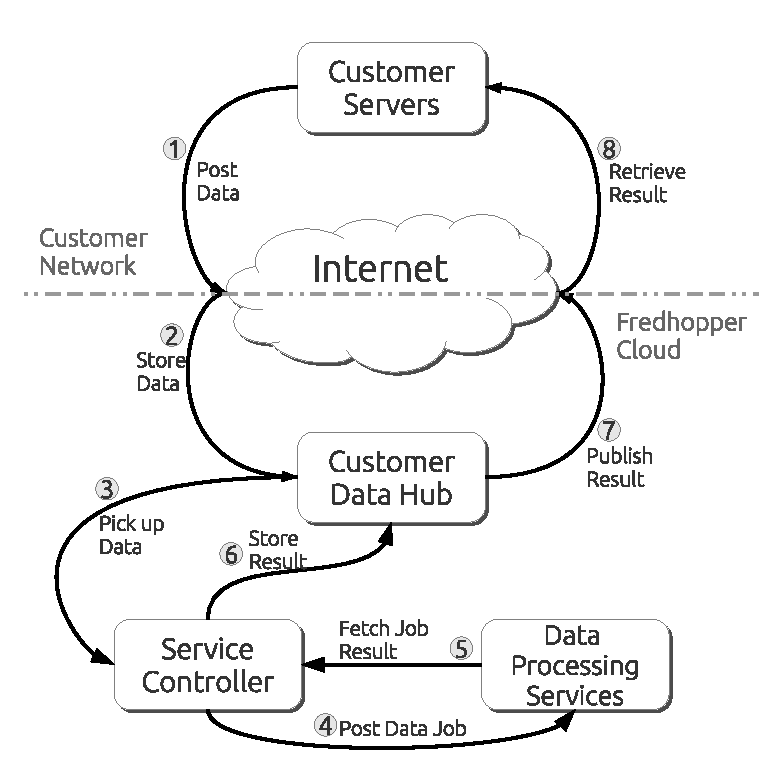
\includegraphics[scale=0.4]{figs/DM}
\end{center}
% \vspace{-20pt}
\caption{Fredhopper's Controller life cycle for remote data processing}
\label{fig:frh-dm}
% \vspace{-10pt}
% \end{wrapfigure}
\end{figure}

Fredhopper is an SDL company since 2008 and a leading search, merchandising and personalization solution provider, whose
products are uniquely tailored to the needs of online business. Fredhopper operates behind the scenes of more than 100 of the largest online
sellers. The Fredhopper Access Server (FAS) provides access to high quality product catalogs.  Typically deployments have about 10
explicit attribute values associated with a product over thousands of attribute dimensions. This challenging task involves working on
difficult issues, such as the performance of information retrieval algorithms, the scalability of dealing with huge amounts of data and
in satisfying large amounts of user requests per unit of time, the fault tolerance of complex distributed systems, and the executive
monitoring and management of large-scale information retrieval operations. Fredhopper offers its services and facilities to e-Commerce
companies (customers) as services (SaaS) over the cloud computing infrastructure (IaaS); which gives rise to different challenges in
regards with resources management techniques and the customer cost model and service level agreements (SLA).

To orchestrate different services such as FAS or data processing, Fredhopper takes advantage of a service controller (a.k.a. Controller).
Controller is responsible to passively manage different service installations for each customer.
For instance, in one scenario, a customer submits their data along with a processing request to their data hub server.
Controller, then picks up the data and initiates a data processing job (usually an ETL job) in a data processing service.
When the data processing is complete, the result is again published to customer environment and additionally becomes available through FAS services.
Figure \ref{fig:frh-dm} illustrates an example scenario that is described above.

In the current implementation of Controller, at Step 4, a data job instance is submitted to a remote data processing service.
Afterwards, the future response of the data job is determined by a periodic remote check on the data service (Step 4). 
When the job is finished, Controller continues to retrieve the data job results (Step 5) and eventually publishes it to customer environment (Step 6).

In terms of system responsiveness, Step 4 may never complete. 
Step 4 failure can have different causes. 
For instance, at any moment of time, there are different customers' data jobs running on one data service node;
i.e. there is a chance that a data service becomes overloaded with data jobs preventing the periodic data job check to return.
If Step 4 fails, it leads the customer into an \emph{unbounded waiting} situation.
According to SLA agreements, this is \emph{not} acceptable.
It is strongly required that for any data job, the customer should be notified of the result: either a completed job with \textsl{success/failed} status, a job that is not completed, or a job with an unknown state.
In other words, Controller should be able to guarantee that any data job request terminates.

To illustrate the contribution of this paper, we extract a closed-world simplified version of the scenario in Figure \ref{fig:frh-dm} from Controller.
In Section \ref{sec:impl}, we provide an implementation-level usage of our work applied to this case study.

\section{Operational Semantics} \label{sec:sos}
We describe the semantics of the language by means of a two-tiered labeled transition system:
a local transition system describes the behavior of a single actor and a global transition system
describes the overall behavior of a system of interacting actors.
We define an actor state as a pair $\langle p,q \rangle$, where
\begin{itemize}
%  \item $o$ is the object identifier
 \item $p$ denotes the current active process of the actor, and
 \item $q$ denotes a queue of pending processes.
\end{itemize}
Each pending process is a pair  $(S, \tau)$ consisting of the current executing statement $S$ and the assignment $\tau$ of 
values  to the  \emph{local} variables (e.g., formal parameters).
The active process consists of a  pair  $(S,\sigma)$, where $\sigma$ assigns values to the local variables
and additionally assigns values to the instance variables
of the actor.



% We use structural approach in operational semantics \cite{plotkin-sos} to present the semantics of application-level scheduling
% with deadlines in Creol. 

% \emph{Object configuration.} We define an object configuration as a pair of $(O, F)$ with $ O = (o, p, q)$ in which:
% \begin{itemize}
%  \item $o$ is the object identifier
%  \item $p$ is the current process of the object that is executing in the single thread of execution for the object. 
%  Each process is a combination $(S, \tau)$ of current executing statement, $S$, and the bindings of both object's internal fields and local variables, $\tau$.
%  \item $q$ is the queue of processes for the object
%  \item $F$ is the bindings of created objects which represents futures; i.e. $F(o)$ denotes a record. 
%  Each record present two propeties; \textsf{val} representing the actual value of a future and \textsf{aborted} if the future has failed.
% \end{itemize}
% 
% \Behrooz{Add time notations for global transition system.}
% \Behrooz{tau can hold the identifier of an object to simplify.}
% \Behrooz{Mention ``run to completion'' for the current process.}

\subsection{Local transition system}
The local transition system defines transitions among actor configurations of the form $\langle p,q,\phi\rangle $,
where $(p,q)$ is an actor state and for any object $o$ identifying a created future,  $\phi$ denotes the shared heap
of the created future objects, i.e., $\phi(o)$, for any future object $o$ existing in $\phi$,  denotes a record with a field
\textsf{val} which represents the return value  and a boolean field \textsf{aborted} which indicates abortion of the process
identified by $o$.

In the local  transition system we make use of the following axiomatization of the occurrence of exceptions.
Here $(S,\sigma,\phi)\uparrow v$ indicates that $S$  raises an exception $v$:
\begin{itemize}\itemsep5pt
 \item $ (x=f.\gett(),\sigma,\phi) \uparrow \sigma(f)$ where $\phi(\sigma(f)).\mathsf{aborted}=\jtt{true}$,
 \item $\frac{\displaystyle (S,\sigma,\phi)\uparrow v}{\trycatch{S}{T}{u}{S'}\uparrow v}$ where $v$ is not of type $\mathsf{T}$, and, 
 \item $\frac{\displaystyle (S,\sigma,\phi)\uparrow v}{\displaystyle (S;S,\sigma,\phi) '\uparrow v}$.
\end{itemize}

We present here the following transitions describing internal computation steps
(we denote by $ \textsf{val}(e)(\sigma)$ the value of the expression $e$ in $\sigma$
and by $f[u\mapsto v]$ the result of assigning the value $v$ to $u$ in the function $f$).

\parbf{Assignment statement} is used to assign a value to a variable:

$$ \langle (x=e; S, \sigma), q, \phi\rangle \rightarrow \langle (S, \sigma [x \mapsto \textsf{val}(e)(\sigma)]), q, \phi\rangle $$

\parbf{Returning a result} consists of setting the field 
\textsf{val} of the future of the process:

$$
\langle (\textbf{\jtt{return}}\; e ;S , \sigma), q, \phi\rangle \rightarrow 
\langle (S, \sigma), q, \phi[\sigma(\jtt{myfuture}).\textsf{val} \mapsto 
\textsf{val}(e)(\sigma)]\rangle
$$

\parbf{Initialization of \jtt{timeout} in \gett  \space operation} 
assigns to a  distinguished (local) variable \jtt{timeout} its initial \emph{absolute} value:
\begin{multline*} \langle  (x=f.\gett(e); S, \sigma), q, \phi\rangle \rightarrow  \\
 \langle (x=f.\gett(e);S, \sigma [\jtt{timeout} \mapsto \textsf{val}(e+\mathsf{time})(\sigma), q, \phi\rangle 
\end{multline*}


\parbf{The \gett \space operation} is used to assign the value of a future to a variable:
$$ \langle  (x=f.\gett(); S, \sigma), q, \phi\rangle \rightarrow \langle (S, \sigma [x \mapsto \phi(\sigma(f)).\mathsf{val}]), q, \phi\rangle $$
where $ \phi(\sigma(f)).\mathsf{val} \neq \bot$ .

\parbf{Timeout} is operationally presented by the following transition:
$$ \langle  (x=f.\gett(); S, \sigma), q, \phi\rangle \rightarrow \langle (S, \sigma), q, \phi\rangle $$
where $\sigma(\jtt{time})< \sigma(\jtt{timeout})$.

\parbf{The \textnormal{\textbf{\jtt{try-catch}}} block} semantics is presented by: 

$$ 
\frac
{\langle (S,\sigma),q, \phi\rangle \rightarrow \langle (S', \sigma'), q', \phi'\rangle}
{\langle (\trycatch{S}{T}{x}{S''};S''', \sigma), q, \phi\rangle \rightarrow \langle (\trycatch{S'}{T}{x}{S''};S''', \sigma), q', \phi'\rangle}
$$ 

\parbf{Exception handling.} 
We provide the operational semantics of exception handling in a general way in the following:
$$
\frac
{(S,\sigma,\phi) \uparrow v}
{\langle (\trycatch{S}{T}{x}{S''};S''', \sigma), q, \phi\rangle \rightarrow \langle  (S'';S''', \sigma[x\mapsto v]), q, \phi\rangle}
$$
where the exception $v$ is  of type \jtt{T}.

\parbf{Abnormal termination} of the active process is generated by an uncaught exception:
$$
\frac
{(S,\sigma,\phi)\uparrow v}
{\langle (S;S', \sigma), q, \phi\rangle \rightarrow \langle (S'',\sigma'), q', \phi'\rangle}
$$
where $q = (S'',\tau) \cdot q' $ and $\sigma'$ is obtained from restoring the values of the local variables
as specified by $\tau$ (formally, $\sigma'(x)=\sigma(x)$, for every instance variable $x$, and $\sigma'(x)=\tau(x)$, for every local variable $x$), and  $\phi'(\sigma(\jtt{myfuture})).\jtt{aborted} = \jtt{true}$
($\phi'(o)=\phi(o)$, for every $o\not= \sigma(\jtt{myfuture})$).

\parbf{Normal termination} is presented by:
$$
\langle (E, \sigma), q, \phi\rangle \rightarrow \langle  (S,\sigma'), q', \phi\rangle
$$
where $q = (S,\tau) \cdot q'$ and $\sigma'$ is obtained from restoring the values of the local variables
as specified by $\tau$ (see above).
We denote by $E$ termination (identifying $S;E$ with $S$).



\parbf{Deadline missed.}
Let  $(S', \tau)$ be some  pending process  in $q$ such that $\tau(\textbf{\jtt{deadline}}) < \sigma(\jtt{time})$.
Then
$$
\langle  (S,\sigma), q, \phi\rangle \rightarrow \langle p, q', \phi'\rangle 
$$
where $q'$ results from $q$ by removing $(S',\tau)$ and $\phi'(\tau(\jtt{myfuture})).\jtt{aborted} = \jtt{true}$
($\phi'(o)=\phi(o)$, for every $o\not= \tau(\jtt{myfuture})$).


\bigskip
% Given a
% method signature $m(\overline{T \: x})$, corresponding incoming messages 
% $o?m(\bar{v})$ and outgoing messages $o!m(\overline{v})$ specify  besides the callee $o$  and the actual values of the specified formal parameters $\bar{x}$
% the values of the variables  $\jtt{myfuture}$ and $\jtt{deadline}$.
% To model locally incoming and outgoing  messages we introduce the following
% labeled transitions.
A message $m(\tau)$ specifies for the method $m$ the  initial assignment $\tau$ of its  local variables
(i.e., the formal parameters and the variables \jtt{this}, \jtt{myfuture}, and \jtt{deadline}).
To model locally incoming and outgoing  messages we introduce the following
labeled transitions.

\parbf{Incoming message.}
Let the active process $p$ belong to the actor $\tau(\jtt{this})$ (i.e., 
 $\sigma(\jtt{this})=\tau(\jtt{this})$ for the assignment $\sigma$ in $p$):
$$
\langle p , q, \phi\rangle \xrightarrow[]{m(\tau)}  \langle p , \mathsf{insert}(q, m(\overline{v}, d)), \phi\rangle
$$
where   $\mathsf{insert}(q, m(\tau))$  defines the result of inserting the process  $(S,\tau)$, where $S$ denotes the body of method $m$,
in $q$, according to some application-specific policy (described below in Section \ref{sec:impl}).


\parbf{Outgoing message.} 
We model an outgoing message by:
$$
\langle (f = e_0 \; ! \; m(\bar{e}) \; \textbf{\jtt{deadline}}(e_1);S,\sigma)  , q, \phi\rangle 
\xrightarrow[]{m(\tau)} 
\langle (S,\sigma[f\mapsto o])  , q, \phi' \rangle 
$$
where 
\begin{itemize}\itemsep5pt
\item $\phi'$ results from $\phi$ by extending its domain  with a new future object $o$
such that $\phi'(o).\textsf{val}=\perp$\footnote{$\perp$ stands for "uninitialized"}and $\phi'(o).\textsf{aborted}=\jtt{false}$,
 \item $\tau(\jtt{this})=\textsf{val}(e_0)(\sigma)$,
 \item $\tau(x)= \textsf{val}(e)(\sigma)$, for every formal parameter $x$ and corresponding actual parameter $e$, 
 \item $\tau(\jtt{deadline})=\sigma(\mathsf{time})+ \textsf{val}(e_1)(\sigma)$,
  \item  $\tau(\jtt{myfuture})=o$.
\end{itemize}

\subsection{Global transition system}
A (global) system configuration $S$ is a pair $(\Sigma, \phi)$ consisting of a set $\Sigma$
of actor states and a global heap $\phi$ which stores the created future objects.
We denote actor states by $s$, $s'$, $s''$, etc.

\parbf{Local computation step.} 
The interleaving of local computation steps of the individual actors is
modeled by the rule:
$$
\frac{(s, \phi) \rightarrow (s', \phi')}
{(\{s\}\cup\Sigma, \phi)\rightarrow (\{s'\}\cup\Sigma, \phi')}
$$

\parbf{Communication.} 
Matching a  message sent by one actor with its  reception by  the specified callee
is described by the rule:
$$
\frac
{(s_1, \phi) \xrightarrow[]{m(\tau)} (s'_1, \phi')\quad (s_2, \phi) \xrightarrow[]{m(\tau)} (s'_2, \phi) }
{(\{s_1,s_2\}\cup\Sigma, \phi) \rightarrow (\{s'_1 , s'_2 \} \cup \Sigma, \phi')}
$$
Note that only an outgoing message affects the shared heap $\phi$ of futures.

\parbf{Progress of Time.}
The following transition uniformly updates the local clocks (represented by the instance variable \jtt{time})
of the actors.
$$
(\Sigma,\phi)\rightarrow (\Sigma',\phi)
$$
where
$$
\Sigma'=\{\langle (S,\sigma'), q, \phi\rangle\mid
\langle (S,\sigma), q, \phi\rangle\in \Sigma,\; \sigma'=\sigma [\jtt{time}\mapsto \sigma(\jtt{time})+\delta]\}
$$
for some positive $\delta$.


% \emph{Time transition.}
% $$
% \langle\mathcal{O}, F, \mathcal{T}\rangle \rightarrow \langle\mathcal{O}, F, \mathcal{T} + \Delta\rangle
% $$
% 
% \emph{Updating a future.}
% 
% $$
% \frac
% {\langle\mathcal{O}, F, \mathcal{T}\rangle \rightarrow \langle\mathcal{O}', F', \mathcal{T} + \Delta\rangle}
% {\langle\{O\} \cup \mathcal{O}, F,\mathcal{T}\rangle \rightarrow \langle\{O'\} \cup \mathcal{O}, F', \mathcal{T} + \Delta\rangle }
% $$



% \subsection{Previously written in case notations would be reused}
% 
% \Behrooz{Previous wrong version. May be removed later.}
% \emph{Receive a new message.} The operational semantics when an object with identifier $o$ receives a message to invoke method $m$ with deadline $d$.
% 
% \begin{align}
% \frac
% {\mathsf{in} = m(\overline{v}, d) + \dot{p} = \mathsf{new()}}
% {(o, (\dot{p}.\jtt{deadline} \mapsto \mathsf{time()} + d,s[\overline{v}], d), p, \mathsf{enq}(q, \dot{p}), \sigma)}
% \end{align}
% 
% in which the operation \textsf{new()} creates a new instance of a process for the concurrent object.
% Additionally, as we discssued in Equation \ref{eq:orderedq}, each concurrent object owns an ordered queue for the processes.
% The process queue is ordered based on the result of $\sigma$ function:
% 
% $$ \sigma(\dot{p}) = \dot{p}.\jtt{deadline} $$
% 
% Thus, the operational semantics of \textsf{enq} ensures to find a proper index place $i$ for the new process $\dot{p}$ such that:
% 
% $$
% \forall k < i \::\: q_k.\jtt{deadline} < \dot{p}.\jtt{deadline} \wedge \forall k > i \::\: q_k.\jtt{deadline} > \dot{p}.\jtt{deadline}
% $$
% 
% And, then, $q_i = \dot{p}$ completes the enqueuing action. Since, $q$ is an \emph{ascending} ordered queue, the required action to deqeue the 
% ``next'' process is simply to remove and return the \emph{head} of the queue; namely $q_0$.
% 
% \emph{Deadline Miss Detection.} A deadline miss is detected by a separate watchdog thread of the active concurrent object.
% The watchdog thread observes all the processes but the current process of the object to allow it complete its execution:
% 
% \begin{align}
% \frac
% {\forall p \neq \overline{p} \::\: (o,s[f_p \mapsto \jtt{null}],\overline{p},q,\sigma) + p.\jtt{deadline} < \mathsf{time()}}
% {(o,s[f_p.\jtt{aborted} \mapsto \jtt{true}], \overline{p}, q - p, \sigma)}
% \end{align}
% 
% Consequently, when the future of a missed-deadline process $p$ is accessed, it causes the application to generate and throw an exception:
% 
% \begin{align}
% \frac
% {(o,(f.\jtt{get()},s[f.\jtt{aborted} = \jtt{true}],d),q,\sigma)}
% {(o,(x \mapsto \jtt{new Exception},s[f \mapsto \jtt{null}],d),q,\sigma)}
% \end{align}

\section{Implementation} \label{sec:impl}
We base our implementation on Java's concurrent package: \jtt{java.util.concurrent}. 
The implementation consists of the following major components:
\begin{enumerate}
 \item An extensible language API that owns the core abstractions, architecture, and implementation. 
For instance, the programmer may extend the concept of a scheduler to take full control of how, i.e., in what order, the processes of the individual actors are queued
(and as such scheduled for execution).
We illustrate the scheduler extensibility with an example in the case study below.
 \item Language Compiler that translates the modeling-level programs into Java source.
 We use ANTLR \cite{antlr} parser generator framework to compile modeling-level programs to actual implementation-level source code of Java.
 \item The language is seamlessly integrated with Java.
 At the time of programming, language abstractions such as data types and third-party libraries from either Crisp or Java are equally usable by the programmer.
\end{enumerate}

We next discuss the underlying deployment of actors and the implementation
of real-time  processes with deadlines.

\parbf{Deploying actors onto JVM threads.}
%As a major improvement to our previous work \cite{crisp-sac}, we changed the model of deployment of actors onto Java threads for simplicity, performance, and better reasoning.
In the implementation, each actor owns a main thread of execution, that is,
the implementation does \emph{not} allocate \emph{one} thread per process because
threads are  \emph{costly} resources and
allocating to each process one thread in general leads to a poor performance:
there can be an arbitrary number of actors in the application and each may receive numerous messages which thus give rise to  a number of threads that  goes beyond the  limits of memory and resources.
Additionally, when processes go into pending mode, their correspondent thread may be reused for other processes.
Thus, for better performance and optimization of resource utilization, the implementation assigns a single thread for all processes inside each actor.

Consequently, at any moment in time, there is only one process that is executed inside each actor.
On the other hand, the actors share a thread which is used
for the execution of a  watchdog for the deadlines of the queued processes (described below) because allocation of such a   thread to each actor  in general slows down the performance.
%Actors take turn in using the shared thread to process and detect possible deadlines on this thread.
Further  this sharing  allows the implementation to decide, based on the underlying resources and hardware, to optimize the allocation of the watchdog thread to actors.
For instance, as long as the resources on the underlying hardware are abundant, the implementation decides to share as less as possible the watchdog thread.
This gives each actor a better opportunity with higher precision to detect missed deadlines.

%\parbf{Implementation of $(S, \tau)$ and $(S, \sigma)$.} 
%As discussed, when an actor receives an incoming message, a process is created for the messages.
%Within the process creation, the process allocates a data structure that behaves as a repository for the process.
%When the process is pending, the process has only access to the local variables and actual parameters of the message.
%When the process is executing, the access is extended to the level of actor's instance variables.
%The access level is managed by Crisp's core architecture when transferring the process from pending state to executing state (and the other way).
%At either state, the process has access to special convenient instances/methods including \jtt{myActor}, \jtt{myFuture}, \jtt{myDeadline};
%respectively, they denote the owning actor for the process, the future that will be the result of the process, and the deadline specified for the process.

\parbf{Implementation of processes with deadlines.}
A process itself is represented in the implementation by a data structure
which encapsulates the values of its local variables and the method to be executed.
Given a relative deadline $d$ as specified by a call
we compute at run-time its absolute deadline (i.e. the expected starting time of the process) by
$$
 \jtt{TimeUnit.toMillis}(d) + \jtt{System.currentTimeMillis()}
$$
which is a \emph{soft} real-time requirement.
%As shown in the above equation, the received deadline is expected to express a \emph{relative} amount of time.
%Each actor maintains a queue of processes to be executed along with the reference to the current executing process.
As in the operational semantics, in the real-time implementation
always the head of the process queue  is scheduled for execution.
This allows the implementation of a \emph{default}
earliest deadline first (EDF) scheduling policy
by  maintaining a queue ordered by  the above absolute time values for the deadlines.

The important consequence of our non-preemptive mode of execution 
for the implementation is the resulting simplicity of thread management
because preemption requires additional thread interrupts that facilitates the abortion of a process in the middle of execution.
% 
As stated above,  a single  thread in the implementation detects if a process has missed its deadline.
This task  runs periodically and to the end of all actors' life span.
%The detection is performed for all processes in the actor's queue (that does not include the current process).
To check for a missed deadline it suffices to simply check  for a process 
that the  above absolute time value of its deadline is \emph{smaller} than
\jtt{System.currentTimeMillis()}.
When a process misses its deadline,  the actions as specified by the corresponding transition of the operational semantics are subsequently performed.
% 
The language API provides  extension points which allow for each actor
the definition of a customized watchdog process and scheduling policy
(i.e., policy for enqueuing processes).
The customized  watchdog processes are still  executed by a single thread.

%In line with our previous work \cite{crisp-sac}, by default, application-level scheduling is realized and implemented using the \jtt{deadline} property of processes.
%In other words, the programmer is able to use asynchronous messages that are extended by deadlines at a higher level to specify application-level scheduling expectations.
%Nonetheless, the programmer still has the flexibility to extend the scheduling API if needed. 
%If the scheduling API is extended by the programmer, they are expected to provide an implementation that is fair in scheduling.
%By fairness, it is expected that no process should enter an unbounded waiting (starvation) state.
%Additionally, the order of processes needs to be determined by the programmer's custom scheduler that can be application specific.

\parbf{Fredhopper case study.}
As introduced in Section \ref{sec:frh}, we extract a closed-world simplified version from Fredhopper Controller.
We apply the approach discussed in this paper to use deadlines for asynchronous messages.
% Controller operates in a high-demand distributed setting as in Figure \ref{fig:ctl:deploy}.

Listing \ref{lst:frh:polling} and \ref{lst:frh:deadlines} present the difference in the previous Controller and the approach in Crisp.
The left code snippet shows the Controller that uses polling to retrieve data processing results.
The right code snippet shows the one that uses messages with deadlines.

\lstset{language=Creol,escapeinside={(*}{*)}} 
\begin{center}
\begin{minipage}[t]{0.48\textwidth}
% \vspace{-25pt}
\begin{lstlisting}[label=lst:frh:polling, caption=With polling]
class DataProcessor begin
	op process(d: Data) ==
		var p := allocDataProcessor(d)
		p ! process (d)
		do {
			s := p ! getStatus (d)
			if (s <> nil)
				var r := p ! getResults(d)
				publishResult(r)
			wait(TimeUnit.toSecond(1))
		} while (true)
end
\end{lstlisting}
\end{minipage}
\hfill
\begin{minipage}[t]{0.48\textwidth}
% \vspace{-25pt}
\begin{lstlisting}[label=lst:frh:deadlines, caption=With deadlines]
class DataProcessor begin
	op process(d: Data) == 
		var p := allocDataProcessor(d)
		var D := estimateDeadline(d)
		var f := 
			p ! process (d) deadline (D)
		try {
			publishResult(f.get())
		} catch (Exception x) {
			if (f.isAborted)
				notifyFailure(d)
		}
end 
\end{lstlisting}
\end{minipage}
% \vspace{-10pt}
\end{center}

% We simplify details in the listing by higher level abstractions using straightforward naming.
% \jtt{Data} is an abstraction for customer data that carries all information required to initiate a data job request on the data processing service.
% Since Controller manages a distributed setting, we need to have \jtt{allocDataProcessor} to find and allocate the proper data processing service node to the current received data.
% Each data processing service understand a service message \jtt{process} that receives and processes the data job.

% In the left snippet, \jtt{getStatus()} and \jtt{getResults()} are operations to fetch the status of a job and publish its results.
% In the right snippet, we need to determine the deadline based on each \emph{customer} job history and size of data; 
% so, we introduce an operation to calculate an estimate of deadline by \jtt{estimateDeadline()}.

When the approach in Crisp in the right snippet is applied to Controller, it is guaranteed that all data job requests are terminated in a \emph{finite} amount of time.
Therefore, there cannot be complains about never receiving a response for a specific data job request.
Many of Fredhopper's customers rely on data jobs to eventually deliver an e-commerce service to their end users.
Thus, to provide a guarantee to them that their job result is always published to their environment is critical to them.
As shown in the code snippet, if the data job request is failed or aborted based on a deadline miss, 
the customer is still eventually informed about the situation and may further decide about it.
However, in the previous version, the customer may never be able to react to a data job request because its results are never published.
% \begin{wrapfigure}{r}{0.35\textwidth}
% \vspace{-35pt}
% \begin{center}
% 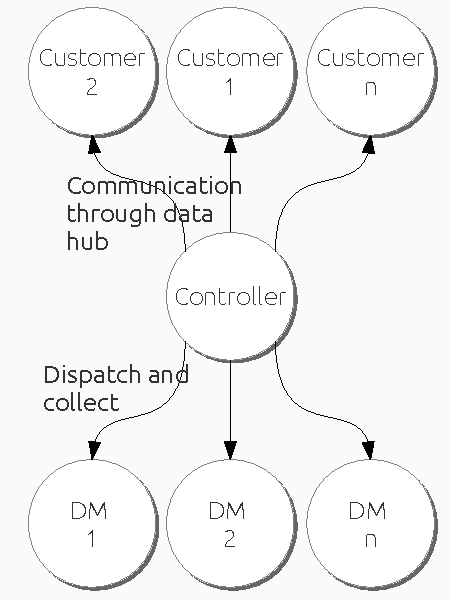
\includegraphics[scale=0.35]{frh-ctl}
% \end{center}
% \vspace{-20pt}
% \caption{Fredhopper's Controller distribution model}
% \label{fig:ctl:deploy}
% \vspace{-15pt}
% \end{wrapfigure}

In comparison to the Controller using polling, there is a way to express timeouts for future values.
However, it does not provide language constructs to specify a deadline for a message that is sent to data processing service.
A deadline may be simulated using a combination of timeout and periodic polling approaches (Listing \ref{lst:frh:polling}).
Though, this approach cannot guarantee eventual termination in all cases; as discussed before that Step 4 in Figure \ref{fig:frh-dm} may never complete.
Controller is required to meet certain customer expectations based on an SLA.
Thus, Controller needs to take advantage of a language/library solution that can provide a higher level of abstraction for real-time scheduling of concurrent messages.
When messages in Crisp carry a deadline specification, Controller is able to guarantee that it can provide a response to the customer.
This termination guarantee is crucial to the business of the customer.

Additionally, on the data processing service node, the new implementation takes advantage of the extensibility of schedulers in Crisp.
As discussed above, the default scheduling policy used for each actor is EDF based on the deadlines carried by incoming messages to the actor.
However, this behavior may be extended and replaced by a custom implementation from the programmer.
In this case study, the priority of processes may differ if they the job request comes from specific customer; i.e.
apart from deadlines, some customers have priority over others because they require a more real-time action on their job requests while others run a more relaxed business model.
To model and implement this custom behavior, a custom scheduler is developed for the data processing node.

\lstset{language=Creol,escapeinside={(*}{*)}} 
\begin{center}
\begin{minipage}[t]{0.48\textwidth}
% \vspace{-30pt}
\begin{lstlisting}[label=lst:frh:dm, caption=Data Processor class]
class DataProcessor begin
	var scheduler := new DataScheduler()
	op process(d: Data) ==
		// do process
end
\end{lstlisting}
\end{minipage}
\hfill
\begin{minipage}[t]{0.48\textwidth}
% \vspace{-30pt}
\begin{lstlisting}[label=lst:frh:sched, caption=Custom scheduler]
class DataScheduler extends DefaultSchedulingManager {
	boolean isPrior(Process p1, Process p2) {
		if (p1.getCustomer().equals("A")) {
			return true;
		}
		return super.isPrior(p1, p2);
	}
}
\end{lstlisting}
\end{minipage}
% \vspace{-15pt}
\end{center}

In the above listings, Listing \ref{lst:frh:sched} defines a custom scheduler that determines the priority of two processes with custom logic for specific customer.
To use the custom scheduler, the only requirement is that the class \jtt{DataProcessor} defines a specific class variable called \jtt{scheduler} in Listing \ref{lst:frh:dm}.
The \textsl{custom scheduler} is picked up by Crisp core architecture and is used to schedule the queued processes.
% In the listing, \jtt{DefaultSchedulingManager} denotes the default EDF scheduler that is implemented in Crisp.
Thus, all processes from customer \jtt{A} have priority over processes from other customers no matter what their deadlines are.

We use Controller's logs for the period of February and March 2013 to examine the evaluation of Crisp approach.
We define \emph{customer satisfaction} as a property that represents the effectiveness of futures with deadline.

\begin{table}[h]
% \begin{wraptable}{l}{0.25\textwidth}
% \vspace{-15pt}
\begin{tabular}{c c}\thickhline
$s_1$ & $s_2$ \\ \thickhline
$88.71\%$ & $94.57\%$ \\ \hline
\end{tabular}
\caption{Evaluation Results}
\label{tbl:eval}
% \vspace{-15pt}
% \end{wraptable}
\end{table}

For a customer $c$, the satisfaction can be denoted by $s = \frac{r^F_c}{r_c}$; in which $r^F_c$ is the number of finished data processing jobs and $r_c$ is the total number of requested data processing jobs from customer $c$. 
We extracted statistics for completed and never-ended data processing jobs from Controller logs ($s_1$).
We replayed the logs with Crisp approach and measured the same property ($s_2$).
We measured the same property for 180 customers that Fredhopper manages on the cloud.
In this evaluation, a total number of about 25000 data processing requests were included.
The results show $6\%$ improvement in Table \ref{tbl:eval} (that amounts to around 1600 better data processing requests). 
Because of data issues or wrong parameters in the data processing requests, there are requests that still fail or never end and should be handled by a human resource.

You may find more information including documentation and source code of Crisp at \surl{http://nobeh.github.com/crisp}.

\section{Related Work} \label{sec:relwork}
The programming language presented in this paper is a real-time  extension of the  language introduced in  \cite{crisp-sac}. This new extension features
\begin{itemize}
 \item integration of  asynchronous messages with  deadlines and futures with timeouts;
 \item  a general mechanism for handling exceptions raised by missed deadlines;
  \item high-level specification of application-level scheduling policies; and
  \item a formal operational semantics.
\end{itemize}
To the best of our knowledge the resulting language is the first implemented 
real-time actor-based programming language which formally integrates the above features.

In several works, e.g,  \cite{ACIHHS11} and \cite{Nielsen96r}, asynchronous messages in actor-based languages are extended with deadlines.
However these languages do not feature futures with timeouts, a general mechanism for handling exceptions raised by missed deadlines or
support the specification of application-level scheduling policies.
Futures and fault handling are considered in the ABS language \cite{abs:2012}.
This work describes recovery mechanisms  for  failed get operations on a future.
However,  the language does not support the specification of real-time requirements,
i.e., no  deadlines for asynchronous messages are  considered and no timeouts on futures.
Further, when a  get operation on a future fails,  \cite{abs:2012} does  not provide any context or information about the exception or the cause for the failure.
Alternatively, \cite{abs:2012} describes  a way to ``compensate'' for a failed get operation on future.
In  \cite{einar:rt:sched:co}, a real-time extension of  ABS with
scheduling policies to model distributed systems is introduced. 
In contrast to Crisp,  Real-Time ABS is an executable  \emph{modeling} language which supports the explicit specification
of the progress of time by means of duration statements for the \emph{analysis} of real-time requirements.
The language does not support however asynchronous messages with  deadlines and futures with timeouts.

%The concurrency model used in this paper is derived from the Actor model enriched by synchronization mechanisms and coupled with strong typing. 
%The Actor model \cite{actors:agha} provides  a suitable formal basis  for multi-core and distributed programming, 
%as objects (actors) are inherently concurrent and autonomous
%entities with a single thread of execution which makes them a natural fit for
%distributed deployment \cite{actor_frameworks_jvm:agha}. 
Two successful examples of actor-based programming languages are Scala and Erlang. 
Scala \cite{scala:actors:ordersky,coord:ordersky} is a hybrid object-oriented and functional programming language inspired by Java. 
% The most important concept introduced in  is that Scala Actors unify
% \textit{thread-based} and \textit{event-based} programming model to fill the gap
% for concurrency programming. 
Through the event-based model, Scala also provides the notion of continuations. Scala further provides  mechanisms for
scheduling of tasks similar to those provided by concurrent Java:
it does not provide a direct and
customizable platform to manage and schedule  messages
received by an individual actor.
Additionally, Akka \cite{akka:homepage} 
extends Scala's actor programming model and as such provides a direct integration with
both Java and Scala. 
% Akka also applies separation of concerns in different 
% aspects of actor programming; it tries to decouple actor model in separate
% including message storage, message dispatching mechanism and message execution.
% It also provides a basic level of message priorities using a simple priority
% generator service.
%To the best of our knowledge neither Scala nor Akka provide a formal operational semantics of the programming language constructs 
%they propose to address the challenges of 
%concurrency, application-level scheduling and real-time requirements.
Erlang \cite{erlang:armstrong} is a dynamically typed functional language that
was developed at Ericsson Computer Science Laboratory with telecommunication
purposes \cite{actors_highly:Correa}. Recent developments in the deployment of
Erlang support the assignment of a scheduler to each processor
\cite{erlang_scheduling} (instead of one global scheduler for the entire
application) but it does not, for example, support application-level scheduling policies.
In general,  none these  languages 
provide  a formally defined real-time extension which integrates the above features.
% This is a crucial improvement in Erlang, because the massive
% number of light-weight processes in the asynchronous setting of Erlang turns
% scheduling into a serious bottleneck. However, the scheduling policies are not
% yet controllable by the application. 

There are well-known efforts in Java to bring in the
functionality of asynchronous message passing onto multicore including Killim
\cite{kilim:Srinivasan:Mycroft}, Jetlang \cite{jetlang}, ActorFoundry
\cite{actor_frameworks_jvm:agha}, and SALSA \cite{salsa:agha}. In
\cite{actor_frameworks_jvm:agha}, the authors present a comparative analysis of
actor-based frameworks for JVM platform. 
Most of these frameworks support futures with timeouts but do not provide asynchronous messages with deadlines, or
a general mechanism for handling exceptions raised by missed deadlines.
Further, pertaining to the domain of
priority scheduling of asynchronous messages, these efforts in general  provide a predetermined
approach or a limited control over message priority scheduling.
As another example, in  \cite{maia_rtsj_11} the use of Java Fork/Join is described  to optimize  mulicore applications.  This work is also based on a \textit{fixed priority} model. 
Additionally, from embedded hardware-software research domain, Ptolemy \cite{ptolemy:lee,actor:lee} is an actor-oriented open architecture and platform that is used to design, model and simulate embedded software. Their approach is hardware software co-design. It provides a platform framework along with a set of tools.

In general, existing high-level programming languages provide the programmer with little real-time control over
scheduling. The state of the art allows specifying priorities for threads or
processes that are  used by the operating system, e.g.,
Real-Time Specification for Java (RTSJ \cite{jsr1,jsr282}) and Erlang. 
Specifically in RTSJ, \cite{zerzel_rtsj} extensively introduces and discusses a framework
for application-level scheduling in RTSJ. It presents a flexible framework to allow scheduling
policies to be used in RTSJ. 
However, \cite{zerzel_rtsj}  addresses the problem mainly in the context of  the standard  multithreading approach to concurrency which in general does not provide
the most suitable approach to distributed applications.
%Thus, all the interesting discussion and extensive features
%relate to the level of \textit{threads} which is not the center of focus in the actor programming model.
In contrast,  in this paper
we have shown that an actor-based  programming
language provides a suitable formal basis for a fully integrated real-time control
in distributed applications.

% The current work contrasts however in the sense that it allows a \textit{fine-grain} and 
% \textit{application-level} scheduling feature in the level of active object with better \textit{flexibility}
% as in the scheduler function.

% Finally, in our previous work, 
% \cite{jaghoori:dating} deals with a real-time extension of a \emph{modeling} language
% based on active objects. In this paper we describe the actual deployment of active objects
% in terms of an implementation of an extension of Java with active objects, using Scala and Akka.
% \cite{crisp-sac} only deals with application-level scheduling policies using priorities.
% In this paper we consider real-time information based on an extension of active objects
% with deadlines and time-outs.

\section{Conclusion and future work} \label{sec:conclusion}
In this paper, we presented both a formal semantics and  an implementation of a real-time actor-based programming language.
We presented how asynchronous messages with deadline can be used to control application-level scheduling with higher abstractions.
We illustrated the language usage with a real-world case study from SDL Fredhopper along the discussion for the implementation.
Currently we are investigating  further optimization of  the implementation of  Crisp and   the formal verification of real-time properties of  Crisp applications using schedulability analysis \cite{sched:elena}.
% Additionally, Crisp targets to support integration with languages that support higher-order abstractions (e.g. Scala).

% \bibliographystyle{plain}
% \bibliography{references}

\lstset{escapeinside={}{}} 
